\documentclass[a4paper,10pt]{article}
\usepackage[utf8]{inputenc}
\usepackage{xspace}
\usepackage{graphicx,graphics} 


%opening
\title{Algorithmic model for N-GREEN optical ring}




\begin{document}

\maketitle

\section*{Definitions, model}
We consider an optical ring composed of $k$ nodes. We can see this ring like $N$ slots rotating to the following position at each time step $t$. The number of slots is given by the length of the ring, and the time step $t$ is the switching granularity. The capacity of a slot depends of the bandwidth of the network (eg, 100 Gbit/s).
\begin{center}   

      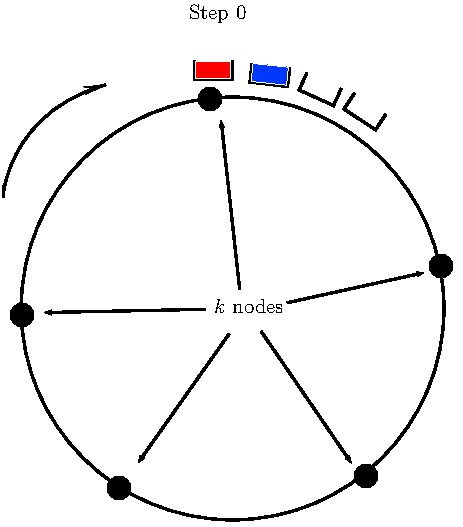
\includegraphics[scale=0.5]{anneau1.pdf}
      \hspace{3cm}
      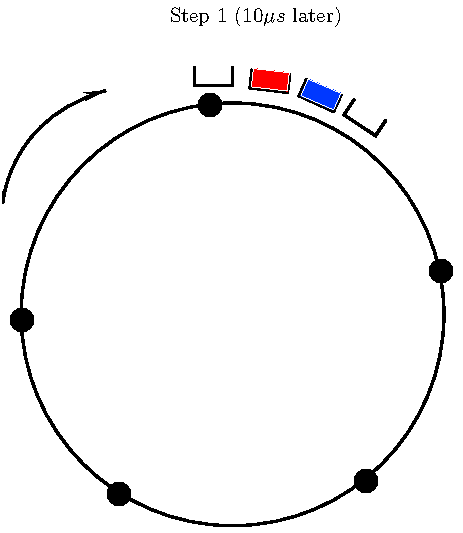
\includegraphics[scale=0.5]{anneau2.pdf}
  
\end{center}
This optical ring is modelled by a graph $G=(V,A)$, in which the vertices in $V$ are the nodes of the ring, and the arcs in $A$ are the links between the nodes. The weight of the arcs is the time taken by a slot to travel the link, i.e. a multiple of $t$. The sum of all the weight of the arcs in the graph in $N$.

\section*{Periodic process}
We define a set $\cal C$ of pair of vertices $(u,v) \in V$. Between each pair of $\cal C$, the following periodic process of period $P$ ($P$ is a multiple of $N$) is observed.
\begin{enumerate}
 \item The node $u$ receives (from an external way) some latency critical data addressed to $v$.
 \item Those data are transferred to $v$ through the ring .
 \item After reception and computing of the message, the node $v$ sends an answer to $u$.
\end{enumerate}
 This periodic process has a critical end to end latency, thus a messages has to be the less buffered as possible before being send in the ring.
 
\section*{Sending policy}

\section*{}
\end{document}